\documentclass[11pt,a4paper]{article}
\usepackage[utf8]{inputenc}
\usepackage[T1]{fontenc}
\usepackage{lmodern}
\usepackage[margin=2.5cm]{geometry}
\usepackage{amsmath,amssymb}
\usepackage{booktabs}
\usepackage{graphicx}
\usepackage{hyperref}
\usepackage{xurl}
\usepackage{setspace}
\onehalfspacing

\hypersetup{
    colorlinks=true,
    linkcolor=blue,
    citecolor=blue,
    urlcolor=blue
}

\title{\textbf{Blockades, Flag Mimicry, and Grain Lifelines: Physical Anatomy of Russian and Baltic Maritime Trade in the Sound Toll Registers, 1700--1856}}

\author{
    Petr Avtonomov\thanks{Independent Researcher, St. Petersburg, Russia. ORCID: \href{https://orcid.org}{0009-0003-2816-6782}. Code and data available at: \url{https://github.com/avtonomov-petr/baltic-sound-toll-anatomy}}
}

\date{\today}

\begin{document}

\maketitle

\begin{abstract}
In a companion study of historical price chronicles (\href{https://doi.org}{Avtonomov, 2026}), we showed that before 1850 European grain markets synchronized episodically around a Baltic--North Sea maritime belt during acute climatic and military emergencies. Yet price chronicles record only market signals; they do not reveal how physical commodities and vessels moved across maritime chokepoints or whether seaborne shipments alleviated local harvest failures. Using the complete digital corpus of the Sound Toll Registers Online (\texttt{STRO}, 1700--1856; 1,274,843 unique ship passages and 3,637,322 cargo records), this paper audits the physical anatomy of Russian and Baltic maritime trade. Systematic orthographic standardization resolves eighteenth-century Danish-German spelling variants and establishes a continuous 135-year benchmark window (1722--1856) following the Treaty of Nystad. Decomposing annual log-growth rates across twenty major ports shows that 37.9\% of total network variance is tightly localized in geopolitical chokepoint closures during the Napoleonic Continental Blockade (1808: 36.8\%; 1814 rebound: 17.5\%) and the Crimean War (1854--1856), yielding a temporal participation ratio of $\mathrm{PR}(u_1) = 0.033$. Removing wartime blockades reduces shared Mode~1 variance to 20.8\% ($\mathrm{PR}(v_1) = 0.539$) and uncovers a structural polarity (Mode~2, 12.6\%) separating a Russian--British industrial-naval belt (St.~Petersburg, Riga, Narva, Vyborg, London, Hull) from a Prussian--Dutch--French grain and wine belt (Gdansk, Stettin, Amsterdam, Rotterdam, Bordeaux). Captain homeport records confirm rapid wartime adaptation: British clearances from St.~Petersburg and Riga fell from 648 in 1806 to zero in 1808 and 1811--1812, partially bridged by neutral U.S.\ vessels (1810--1811) and followed by a sixfold post-1814 surge in Russian Baltic flags. Finally, linking physical grain passages to eighteenth- and nineteenth-century famine crises reveals a regime shift from supply-side contractions in 1741, 1771, and 1795 (204--436 grain ships) to massive Russian export lifelines in 1817 (2,630 ships) and 1847 (3,263 ships, led by 1,275 clearances from St.~Petersburg).
\end{abstract}

\noindent\textbf{Keywords:} economic history, Baltic trade, Sound Toll Registers, Russian Empire, Continental Blockade, grain trade, spectral analysis, archival data audit.

\section{Introduction}

How do maritime chokepoints transmit—or absorb—economic and geopolitical shocks, and how do physical trade flows relate to the price signals observed in historical markets? In a preceding study of high-density price chronicles from the Allen--Unger database (\href{https://doi.org}{Avtonomov, 2026}), we demonstrated that before the mid-nineteenth-century steam revolution, European grain prices co-moved primarily within a Baltic--North Sea--Channel maritime belt and synchronized episodically during acute climatic and military emergencies rather than through continuous peacetime arbitrage. Price series, however, capture only equilibrium valuations; they leave open the physical logistics behind those signals. Specifically, when grain prices spiked across Western Europe during eighteenth- and nineteenth-century famines, did physical grain shipments out of the Baltic expand to relieve Western shortages, or did harvest failures and wartime blockades simultaneously choke off maritime supply?

For nearly a century, quantitative scholarship on Baltic commerce relied on the monumental printed summary tables compiled by Nina Ellinger Bang and Knud Korst (1906--1953). While indispensable, those aggregate tabulations ended in 1783—omitting the French Revolutionary and Napoleonic Wars, the Continental Blockade (1807--1812), and the early steam transition—and severed the relational link between a vessel's port of departure, its cargo composition, and the homeport of its shipmaster. The complete digitization of the Danish Sound Toll Registers Online (\texttt{STRO}; Veluwenkamp \& Scheltjens, 2018) transforms this empirical landscape by preserving individual passage and cargo records through the Øresund strait between Elsinore and Helsingborg up to the abolition of the Sound dues in 1857.

This paper applies a reproducible archival pre-audit and two-tier spectral decomposition to the consolidated \texttt{STRO} database over 1700--1856, placing the emergence of Russia's Baltic ports—above all St.~Petersburg and Riga—within the wider European maritime network. Classic world-systems historiography (Wallerstein, 1980) portrayed the Baltic and Russia as a homogeneous raw-material periphery driven passively by Dutch and British demand, whereas revisionist maritime historians have emphasized regional specialization, institutional resilience, and neutral-flag adaptation during wartime blockades (van Tielhof, 2002; Kotilaine, 2005; Scheltjens, 2015).

By auditing 1,274,843 unique passages and 3,637,322 cargo entries, we establish three empirical findings:
\begin{enumerate}
    \item \textbf{Geopolitical Localization versus Peacetime Structure:} Across twenty core ports over 1722--1856, nearly two-fifths of annual log-growth variance (37.9\%) is concentrated in physical chokepoint closures during the Napoleonic Wars (1807--1814) and the Crimean War (1854--1856), yielding an extreme temporal localization ($\mathrm{PR}(u_1) = 0.033$). Once wartime blockades are removed, shared Mode~1 variance falls to 20.8\% ($\mathrm{PR}(v_1) = 0.539$), revealing a persistent structural polarity (Mode~2, 12.6\%) between a \emph{Russian--British industrial-naval belt} (hemp, flax, bar iron, tallow, timber) and a \emph{Prussian--Dutch--French grain and wine belt}.
    \item \textbf{Wartime Blockades and Flag Mimicry:} Tracking shipmaster homeports on departures from St.~Petersburg and Riga documents the immediate severance of direct British shipping during the Anglo-Russian War (falling from 648 clearances in 1806 to zero in 1808 and 1811--1812, and from 600 in 1853 to one per year in 1854--1855), alongside tactical substitution via neutral U.S.\ vessels in 1810--1811 and an enduring expansion of Russian Baltic-registered shipping after 1814.
    \item \textbf{From Eighteenth-Century Supply Contractions to Nineteenth-Century Grain Lifelines:} Linking physical grain-carrying passages to the famine crises identified in our companion price study reveals a decisive structural reversal. During eighteenth-century crises (1741, 1771, and 1795), physical grain clearances from six core Baltic ports collapsed to 204--436 ships per year (well below the 1729--1855 mean of 774), reflecting synchronized harvest failures and export embargoes. In the nineteenth century, by contrast, Baltic and Russian ports acted as elastic supply lifelines, dispatching 2,630 grain ships during the post-Tambora crisis of 1817 and 3,263 ships during the European subsistence crisis of 1847, when St.~Petersburg alone cleared 1,275 grain vessels.
\end{enumerate}

\section{Archival Pre-Audit and Data Architecture}

\subsection{Relational Structure and Orthographic Standardization}
The raw \texttt{STRO} release comprises two relational tables linked by a unique passage identifier (\texttt{id\_doorvaart}): the passage register (\texttt{doorvaarten.csv}, containing 2,152,670 total records from 1497 to 1857, including date, shipmaster name, and shipmaster homeport \texttt{schipper\_plaatsnaam}) and the cargo register (\texttt{ladingen.csv}, containing 5,568,590 commodity lines detailing departure port \texttt{van}, destination port \texttt{naar}, unit of measurement \texttt{maat}, quantity \texttt{aantal}, and commodity description \texttt{soort}). Restricting the audit to the period 1700--1856 ($T = 157$ calendar years) yields 1,274,843 unique ship passages and 3,637,322 cargo entries with zero missing calendar years.

A foundational requirement of historical data auditing is resolving pre-standardization orthographic fragmentation before aggregating series. In the \texttt{STRO} records, Danish and German customs clerks recorded identical ports and commodities under dozens of phonetic variants. Without systematic normalization, major commercial hubs are artificially split across disconnected strings: St.~Petersburg appears under \texttt{Petersborg} (177,633 cargo rows), \texttt{St.\ Petersborg} (91,494), \texttt{Ste.\ Petersborg} (4,460), \texttt{Petersburg} (945), and \texttt{Petersb.} (819), totaling 279,477 commodity entries; Gdansk is split across \texttt{Dantzig} (199,072), \texttt{Danzig} (92,242), \texttt{Danschen} (55,641), and \texttt{Danschenn} (13,915); and Amsterdam appears under \texttt{Amsterdam} (376,546) and \texttt{Amsterd.} (99,983). Similarly, rye is divided between \texttt{Rug} (157,767) and \texttt{Rugh} (51,359), wheat between \texttt{Hvede} (70,345) and \texttt{Huede} (39,090), and bar iron across \texttt{Jern}, \texttt{Stangjern}, and \texttt{Stang jern}.

To prevent false aggregations and multi-port double counting, our pre-audit pipeline applies three strict filtering rules:
\begin{enumerate}
\item \textbf{Exclusion of Compound Itineraries and Homonyms:} Departure strings indicating sequential multi-port voyages (e.g., \texttt{Petersborg og Wyborg}, \texttt{Riga sidst fra Kjøbenhavn}) are excluded so that each passage is attributed to a single primary port of loading. False lexical matches such as \texttt{Londonderry} (matched against \texttt{London}) and \texttt{Ny Archangel} (Sitka in Russian America, matched against \texttt{Archangel}) are explicitly filtered out.
\item \textbf{Passage-Level Deduplication:} Because a single vessel carrying five distinct cargo lots generates five rows in \texttt{ladingen.csv}, port activity is measured by deduplicating on \texttt{(id\_doorvaart, dep\_clean)}, ensuring each ship passage is counted once per departure port.

\item \textbf{Geographic Boundary Audit:} Screening all Russian ports reveals that Arkhangelsk accounts for only 290 passages through the Sound over 1700--1856, because White Sea commerce with Britain and the Dutch Republic sailed around the North Cape without entering the Danish straits. Consequently, the Russian maritime interface in \texttt{STRO} is anchored in seven Baltic ports: Riga (81,518 unique outbound passages), St.~Petersburg (72,536), Narva (13,543), Vyborg (8,110), Libau/Windau (7,326), Pernau (4,419), and Reval (1,750).
\end{enumerate}
\subsection{Establishing the 1722--1856 Benchmark Window}
Tracking early departures from St.~Petersburg confirms the physical timing of Russia's Baltic integration. Between 1703 and 1709, during the initial construction of the city and Swedish naval blockades of the Gulf of Finland, zero outbound passages from St.~Petersburg are recorded in \texttt{STRO}. A single vessel cleared in 1710, followed by intermittent wartime clearances between 1713 and 1721 (peaking at 59 ships in 1715 and 21 in 1721). Immediately following the Treaty of Nystad (1721) and the protective Russian customs tariff of 1724, outbound traffic surged to 85 ships in 1722, 107 in 1723, 100 in 1724, and 145 in 1725. Over the full 1700--1856 period, St.~Petersburg ranked fourth among all European departure ports in the Sound, behind only Riga (81,518), Amsterdam (80,040), and Gdansk (76,219), and ahead of London (59,614) and Copenhagen (53,434).
Starting the core network panel in 1722 ($T = 135$ years, 1722--1856) yields a dense, continuous matrix across $N = 20$ major ports: seven Russian Baltic ports (\texttt{St\_Petersburg}, \texttt{Riga}, \texttt{Narva}, \texttt{Vyborg}, \texttt{Libau\_Windau}, \texttt{Pernau}, \texttt{Reval}), five Prussian and Mecklenburg ports (\texttt{Gdansk}, \texttt{Konigsberg}, \texttt{Memel}, \texttt{Stettin}, \texttt{Rostock}), three Scandinavian hubs (\texttt{Stockholm}, \texttt{Gothenburg}, \texttt{Copenhagen}), and five Western European ports (\texttt{Amsterdam}, \texttt{Rotterdam}, \texttt{London}, \texttt{Hull}, \texttt{Bordeaux}). Across these 135 years, core ports exhibit zero missing years except during the physical blockade of the Øresund in 1808. To accommodate zero-passage blockade years without arbitrary trimming, we analyze standardized annual log-growth rates $\Delta \ln(1 + X_{t,j})$ over $M = 134$ annual transitions.

\section{Empirical Results}
\subsection{Geopolitical Chokepoint Localization versus Peacetime Trade Structure}
Applying singular value decomposition and participation ratio diagnostics (Appendix~A) to the 20-port log-growth matrix over 1722--1856 reveals a striking dichotomy between wartime chokepoint shocks and peacetime commercial rhythms (Table~\ref{tab:summary} and Figure~\ref{fig:fig1}). In the full 134-transition sample, Mode~1 accounts for 37.9\% of total variance and spans almost the entire port network ($\mathrm{PR}(v_1) = 0.854$, with leading energy shares in Riga at 8.63\%, Hull at 7.61\%, St.~Petersburg at 7.38\%, Amsterdam at 7.30\%, and Narva at 7.17\%). However, the temporal participation ratio is exceptionally low at $\mathrm{PR}(u_1) = 0.033$ (95\% CI: $[0.020, 0.066]$). Inspection of squared temporal scores $u_{t,1}^2$ (Figure~\ref{fig:fig1}B) demonstrates that 73.2\% of Mode~1's temporal energy is concentrated in just seven crisis transitions associated with the Napoleonic Wars and Continental Blockade—led by the closure of the Sound in 1808 (36.76\% of Mode~1 energy) and the post-Napoleonic reopening surge in 1814 (17.51\%), alongside 1807 (7.37\%) and 1810 (6.59\%)—plus the Crimean War blockade and rebound of 1854--1856 (12.38\% combined). Within the seven-port Russian sub-panel, these two naval blockades account for 60.8\% of total annual variance ($\mathrm{PR}(u_1) = 0.032$).

\begin{table}[htbp]
\centering
\caption{Summary of Baltic and Russian Maritime Network Synchronization (1722--1856)}
\label{tab:summary}
\resizebox{\textwidth}{!}{%
\begin{tabular}{lccccc}
\toprule
\textbf{Network Panel} & \textbf{Trans. ($M$)} & \textbf{Mode 1 Var.} & \textbf{Temporal $\mathrm{PR}(u_1)$} & \textbf{Spatial $\mathrm{PR}(v_1)$} & \textbf{Graph Split ($p$-val)} \\
\midrule
Full 20-Port Network & 134 & 37.9\% & 0.033 [0.020, 0.066] & 0.854 [0.704, 0.877] & 1775 ($p = 0.350$) \\
Peace-Time 20-Port (excl.\ blockades) & 123 & 20.8\% & 0.133 [0.095, 0.188] & 0.539 [0.500, 0.573] & 1836 ($p = 0.231$) \\
Russian 7-Port Sub-Panel (Full) & 134 & 60.8\% & 0.032 & 0.867 & --- \\
Russian 7-Port Sub-Panel (Peace) & 123 & 28.2\% & 0.259 & 0.718 & --- \\
\bottomrule
\end{tabular}%
}
\vspace{1mm}
\begin{minipage}{\textwidth}
\footnotesize\emph{Notes:} Calculations performed on standardized annual log-differences $\Delta \ln(1 + X_{t,j})$ of unique outbound ship passages. Brackets report 95\% subsampling bootstrap confidence intervals (300 draws at 80\% sample length). Peace-time panels exclude the Napoleonic blockade and post-war rebound (1807--1814) and the Crimean War closure and rebound (1854--1856). Graph split reports the candidate regime boundary minimizing the Mann--Whitney $U$ $p$-value on the symmetric $k$-NN Laplacian Fiedler vector $\psi_2$ ($k=8$).
\end{minipage}
\end{table}


\begin{figure}[htbp]
\centering
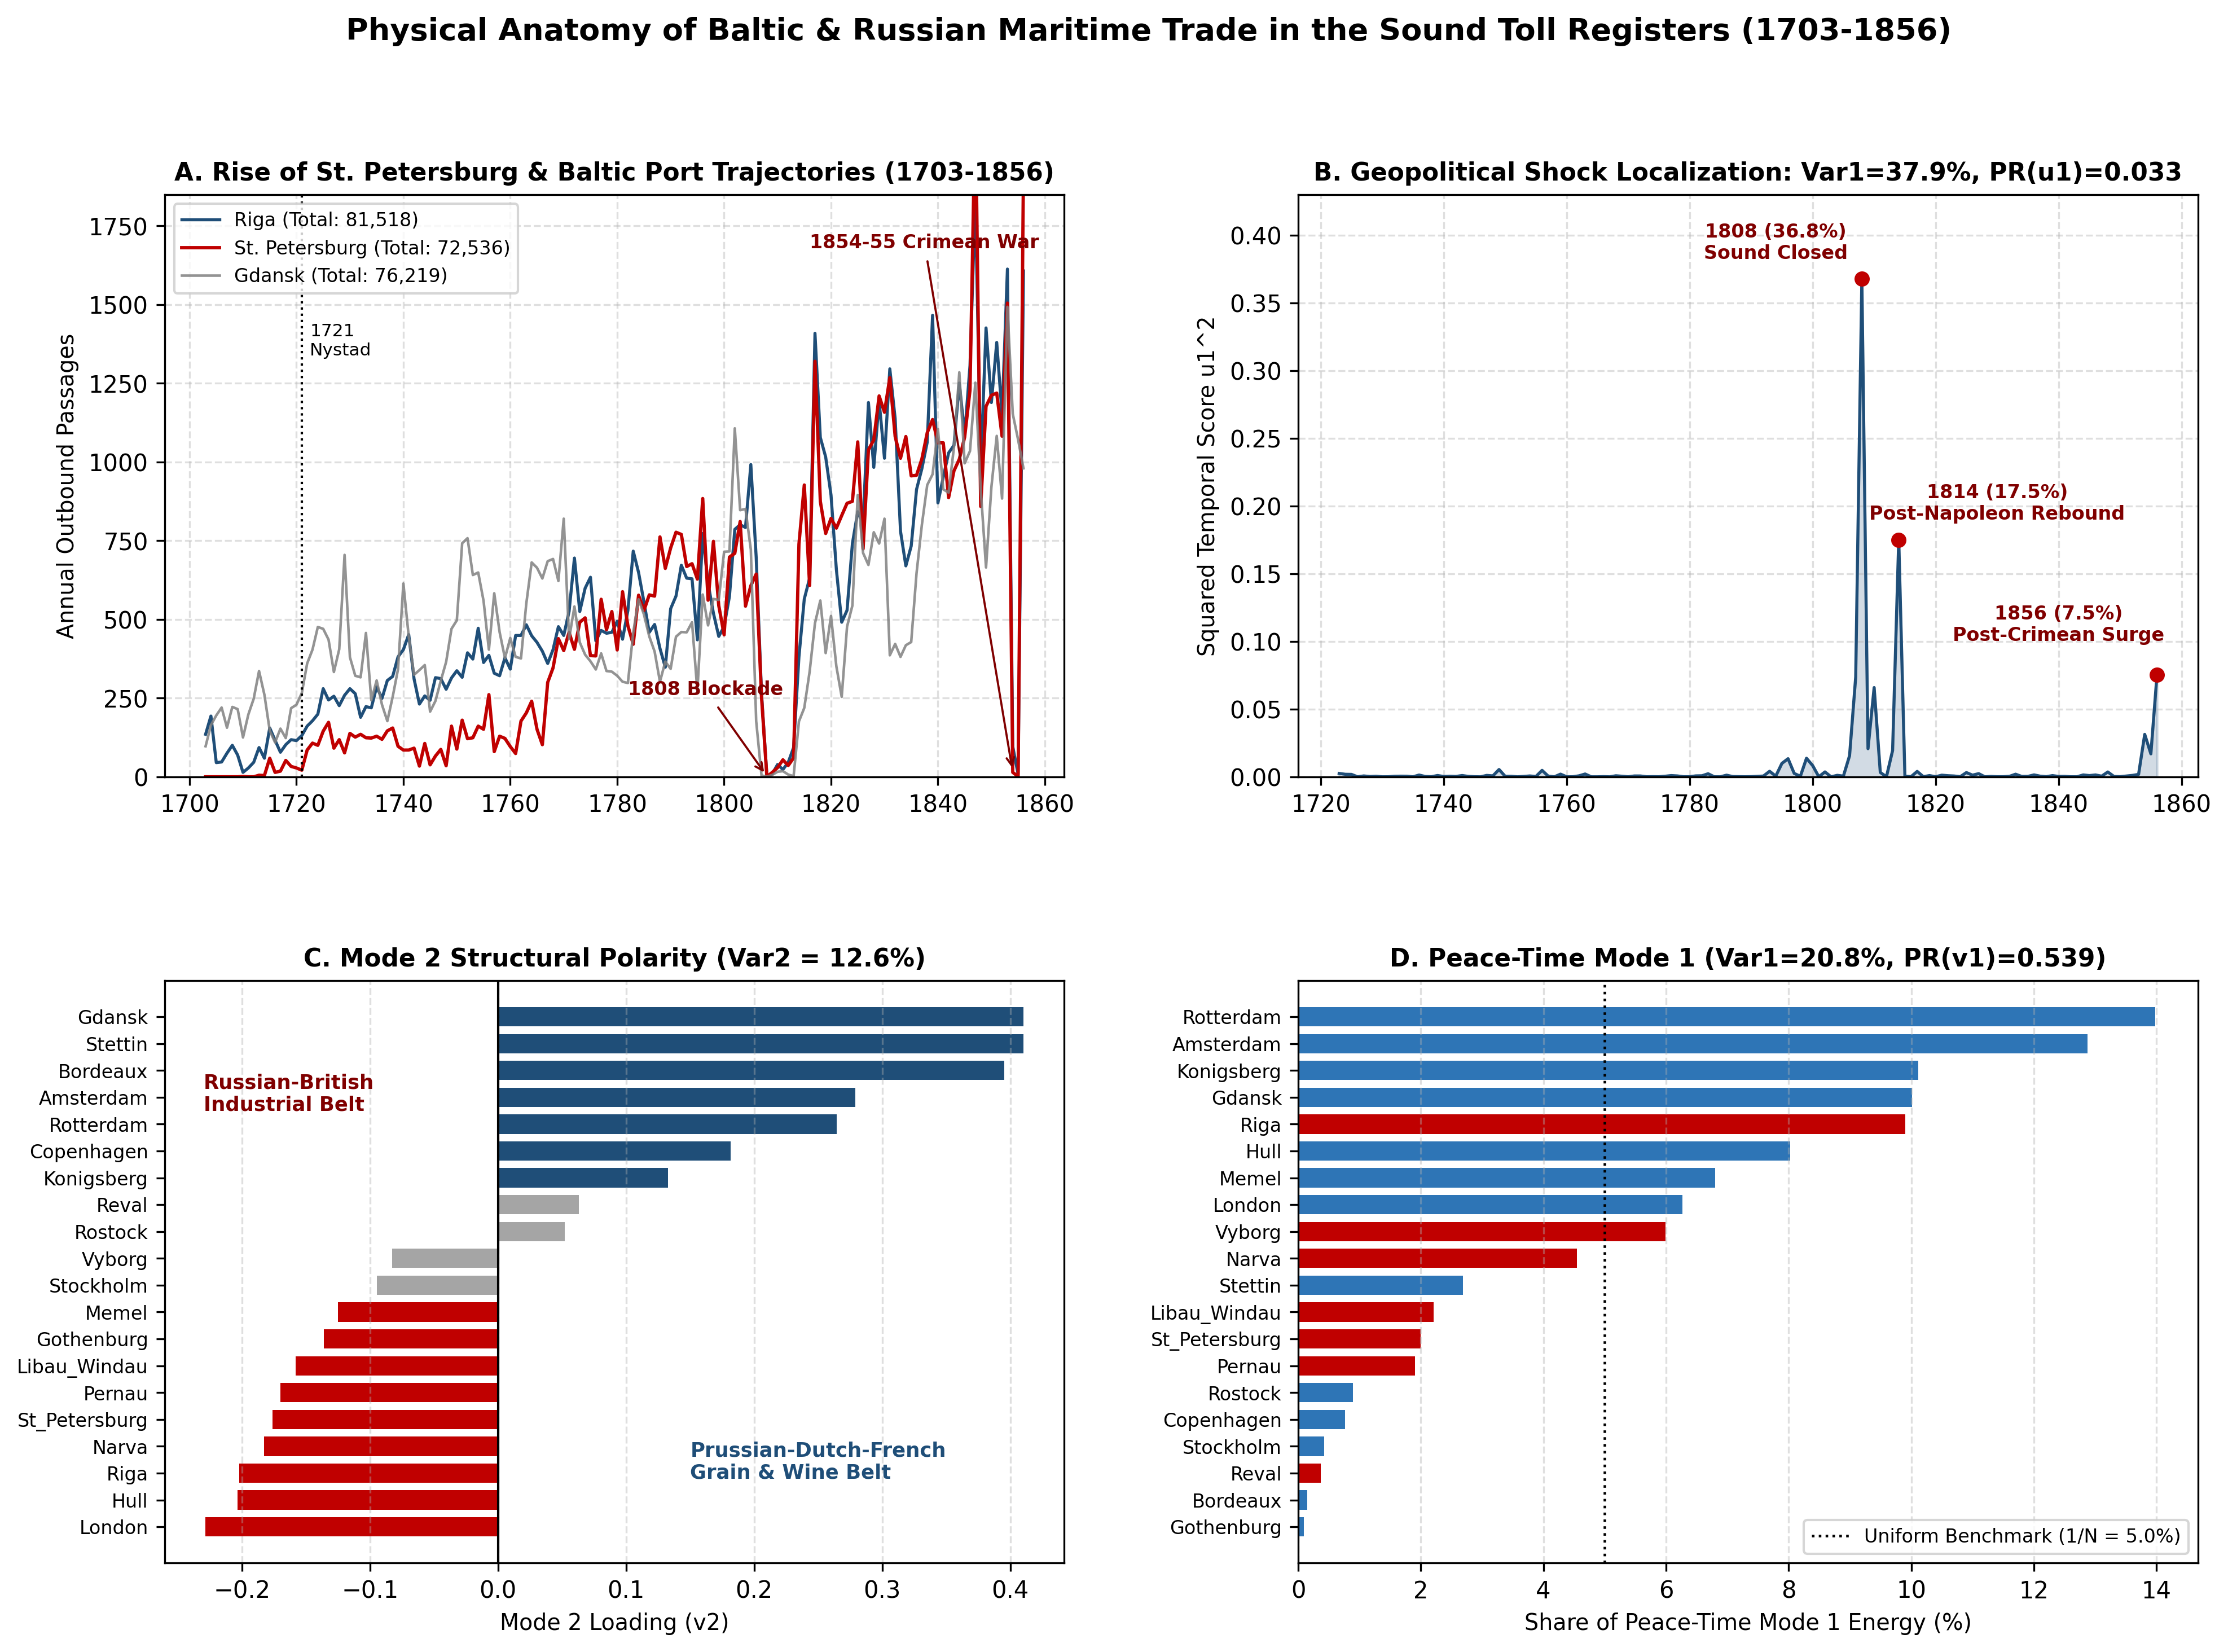
\includegraphics[width=\textwidth]{Figure_1_STRO.png}
\caption{\textbf{Physical Anatomy of Baltic and Russian Maritime Trade (1703--1856).} \textbf{A:} Annual outbound passages from Riga, St.~Petersburg, and Gdansk following the Treaty of Nystad (1721). \textbf{B:} Temporal localization of Mode~1 energy ($u_{t,1}^2$), showing dominance of the 1808 blockade, 1814 reopening, and 1854--1856 Crimean War. \textbf{C:} Mode~2 cross-sectional loadings ($v_{j,2}$), contrasting the Russian--British industrial-naval belt (negative loadings) against the Prussian--Dutch--French grain and wine belt (positive loadings). \textbf{D:} Peacetime Mode~1 energy shares after removing 1807--1814 and 1854--1856.}
\label{fig:fig1}
\end{figure}

Removing the eleven war-blockade and immediate rebound transitions (1807--1814 and 1854--1856, leaving $M = 123$ peacetime transitions) fundamentally alters the network topology (Figure~\ref{fig:fig1}D). Shared Mode~1 variance drops by nearly half to 20.8\%, and cross-sectional participation contracts from 0.854 to $\mathrm{PR}(v_1) = 0.539$ ($[0.500, 0.573]$). In peacetime, annual fluctuations are governed by a North Sea--Southern Baltic commercial core led by Rotterdam (13.98\% of Mode~1 energy), Amsterdam (12.88\%), Konigsberg (10.11\%), Gdansk (10.01\%), Riga (9.90\%), and Hull (8.03\%)—the exact maritime arc identified in our companion price study (\href{https://doi.org}{Avtonomov, 2026}). By contrast, St.~Petersburg contributes only 2.00\% to peacetime Mode~1 variance (well below the 5.00\% uniform benchmark), indicating that its industrial-raw-material shipments moved on multi-year naval and mercantile contracts rather than short-term harvest fluctuations.

Furthermore, Mode~2 of the full panel (12.6\% of variance; Figure~\ref{fig:fig1}C) uncovers a clean structural polarity across the twenty ports. Every Russian port (\texttt{Riga} $-0.202$, \texttt{Narva} $-0.183$, \texttt{St\_Petersburg} $-0.176$, \texttt{Pernau} $-0.170$, \texttt{Libau\_Windau} $-0.158$, \texttt{Vyborg} $-0.083$) clusters on the negative pole alongside Britain (\texttt{London} $-0.228$, \texttt{Hull} $-0.203$) and Sweden (\texttt{Stockholm} $-0.095$), whereas the positive pole is anchored by \texttt{Gdansk} ($+0.410$), \texttt{Stettin} ($+0.410$), \texttt{Bordeaux} ($+0.395$), \texttt{Amsterdam} ($+0.279$), \texttt{Rotterdam} ($+0.264$), \texttt{Copenhagen} ($+0.181$), and \texttt{Konigsberg} ($+0.133$). Meanwhile, the second-echelon transition graph scan detects no statistically significant internal regime break within 1722--1856 ($p = 0.350$ for the full sample; $p = 0.231$ in peacetime), confirming that once St.~Petersburg entered the network in 1722, the underlying structural division of labor persisted until the abolition of the Sound dues.

\subsection{Commodity Specialization and Wartime Flag Adaptation}
Disaggregating cargo records across seven major export hubs over 1722--1856 explains the economic basis of this two-belt polarity (Figure~\ref{fig:fig2}A). St.~Petersburg functioned as the Baltic's premier industrial and naval-stores hub: bar iron accounted for 11.1\% of all recorded cargo lots (nearly twenty times the share in Riga or Gdansk), hemp and flax for 24.6\%, and tallow and potash for 9.9\%, whereas grain represented just 3.1\%. Riga specialized overwhelmingly in hemp and flax (51.1\% of all cargo entries) alongside timber and tar (16.4\%) and grain (7.5\%). Narva (47.6\%), Vyborg (45.7\%), and Memel (40.8\%) operated as specialized timber-exporting ports, while Konigsberg (29.1\% grain, 29.0\% flax/hemp) and Gdansk (19.2\% grain, 20.7\% timber) formed the southern Baltic breadbasket.

\begin{figure}[htbp]
\centering
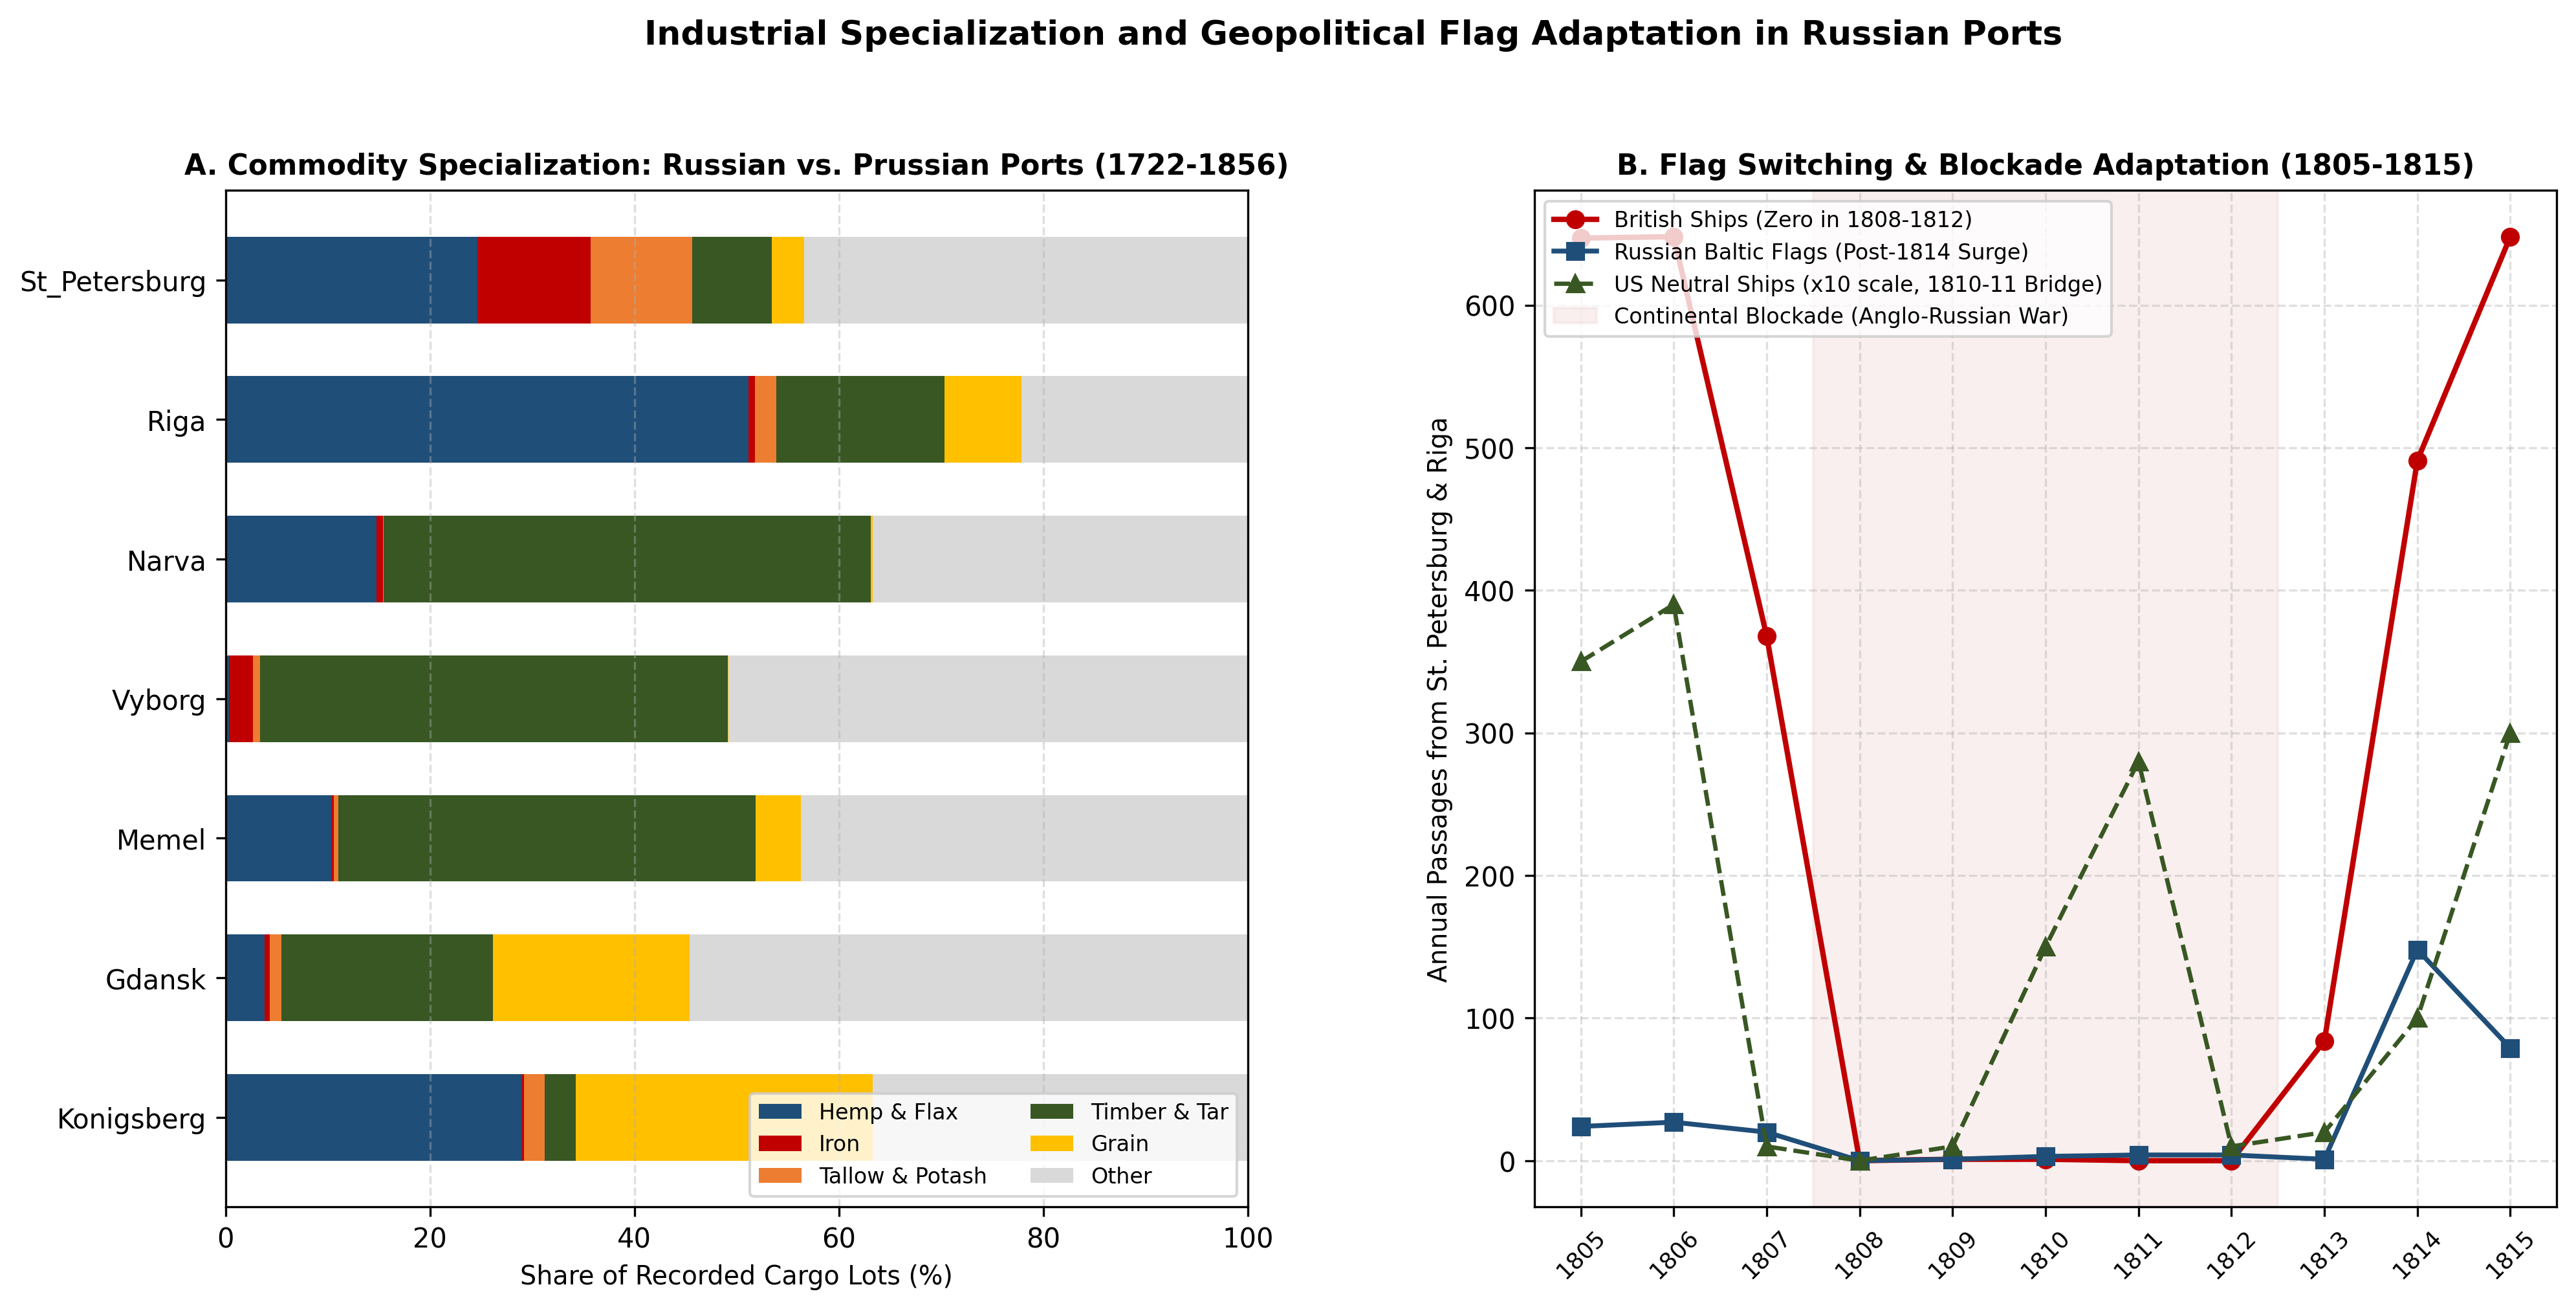
\includegraphics[width=\textwidth]{Figure_2_STRO.png}
\caption{\textbf{Industrial Specialization and Geopolitical Flag Adaptation in Russian Ports.} \textbf{A:} Commodity composition of recorded cargo lots across Russian and Prussian ports (1722--1856). \textbf{B:} Shipmaster homeport registry on outbound passages from St.~Petersburg and Riga during the Napoleonic era (1805--1815), illustrating the disappearance of British flags in 1808--1812, the neutral U.S.\ shipping bridge in 1810--1811, and the post-1814 surge in Russian Baltic flags.}
\label{fig:fig2}
\end{figure}

Classifying shipmaster homeports (\texttt{schipper\_plaatsnaam}, including Scottish and English outports such as Montrose, Arbroath, Shields, Aberdeen, and Dundee) on outbound passages from St.~Petersburg and Riga exposes the mechanics of wartime adaptation (Figure~\ref{fig:fig2}B). In 1805 and 1806, British-homed vessels accounted for 647 and 648 clearances per year from St.~Petersburg and Riga. Following the Treaty of Tilsit and the outbreak of the Anglo-Russian War in late 1807, British clearances dropped to 368 in 1807 and fell to zero in 1808, 1811, and 1812 (with only single isolated entries in 1809--1810). During this blockade window, trade adapted along two channels: first, neutral American vessels (\texttt{Boston}, \texttt{New York}, \texttt{Salem}, \texttt{Philadelphia}, \texttt{Baltimore}) surged from 1 ship in 1807--1809 to 15 in 1810 and 28 in 1811, providing an indirect neutral bridge for Russian hemp and iron; second, immediately upon the reopening of Baltic trade in 1814, vessels registered to Russian Baltic homeports jumped nearly sixfold above pre-war levels (from 24--27 clearances in 1805--1806 to 148 in 1814). An analogous rupture occurred during the Crimean War, when British clearances from St.~Petersburg and Riga dropped from 600 in 1853 to a single vessel per year in 1854--1855 before rebounding to 503 in 1856.


\subsection{Bridging Prices and Physical Flows: Grain Lifelines in European Crises}
Finally, isolating grain-carrying vessels (rye, wheat, barley, and oats) departing from six core Baltic ports (\texttt{Gdansk}, \texttt{Konigsberg}, \texttt{Riga}, \texttt{St\_Petersburg}, \texttt{Memel}, and \texttt{Stettin}) between 1729 and 1855 ($N = 98,241$ total grain passages; long-run average of 774 ships per year) resolves the relationship between price spikes and physical trade (Figure~\ref{fig:fig3}).
\begin{figure}[htbp]
\centering
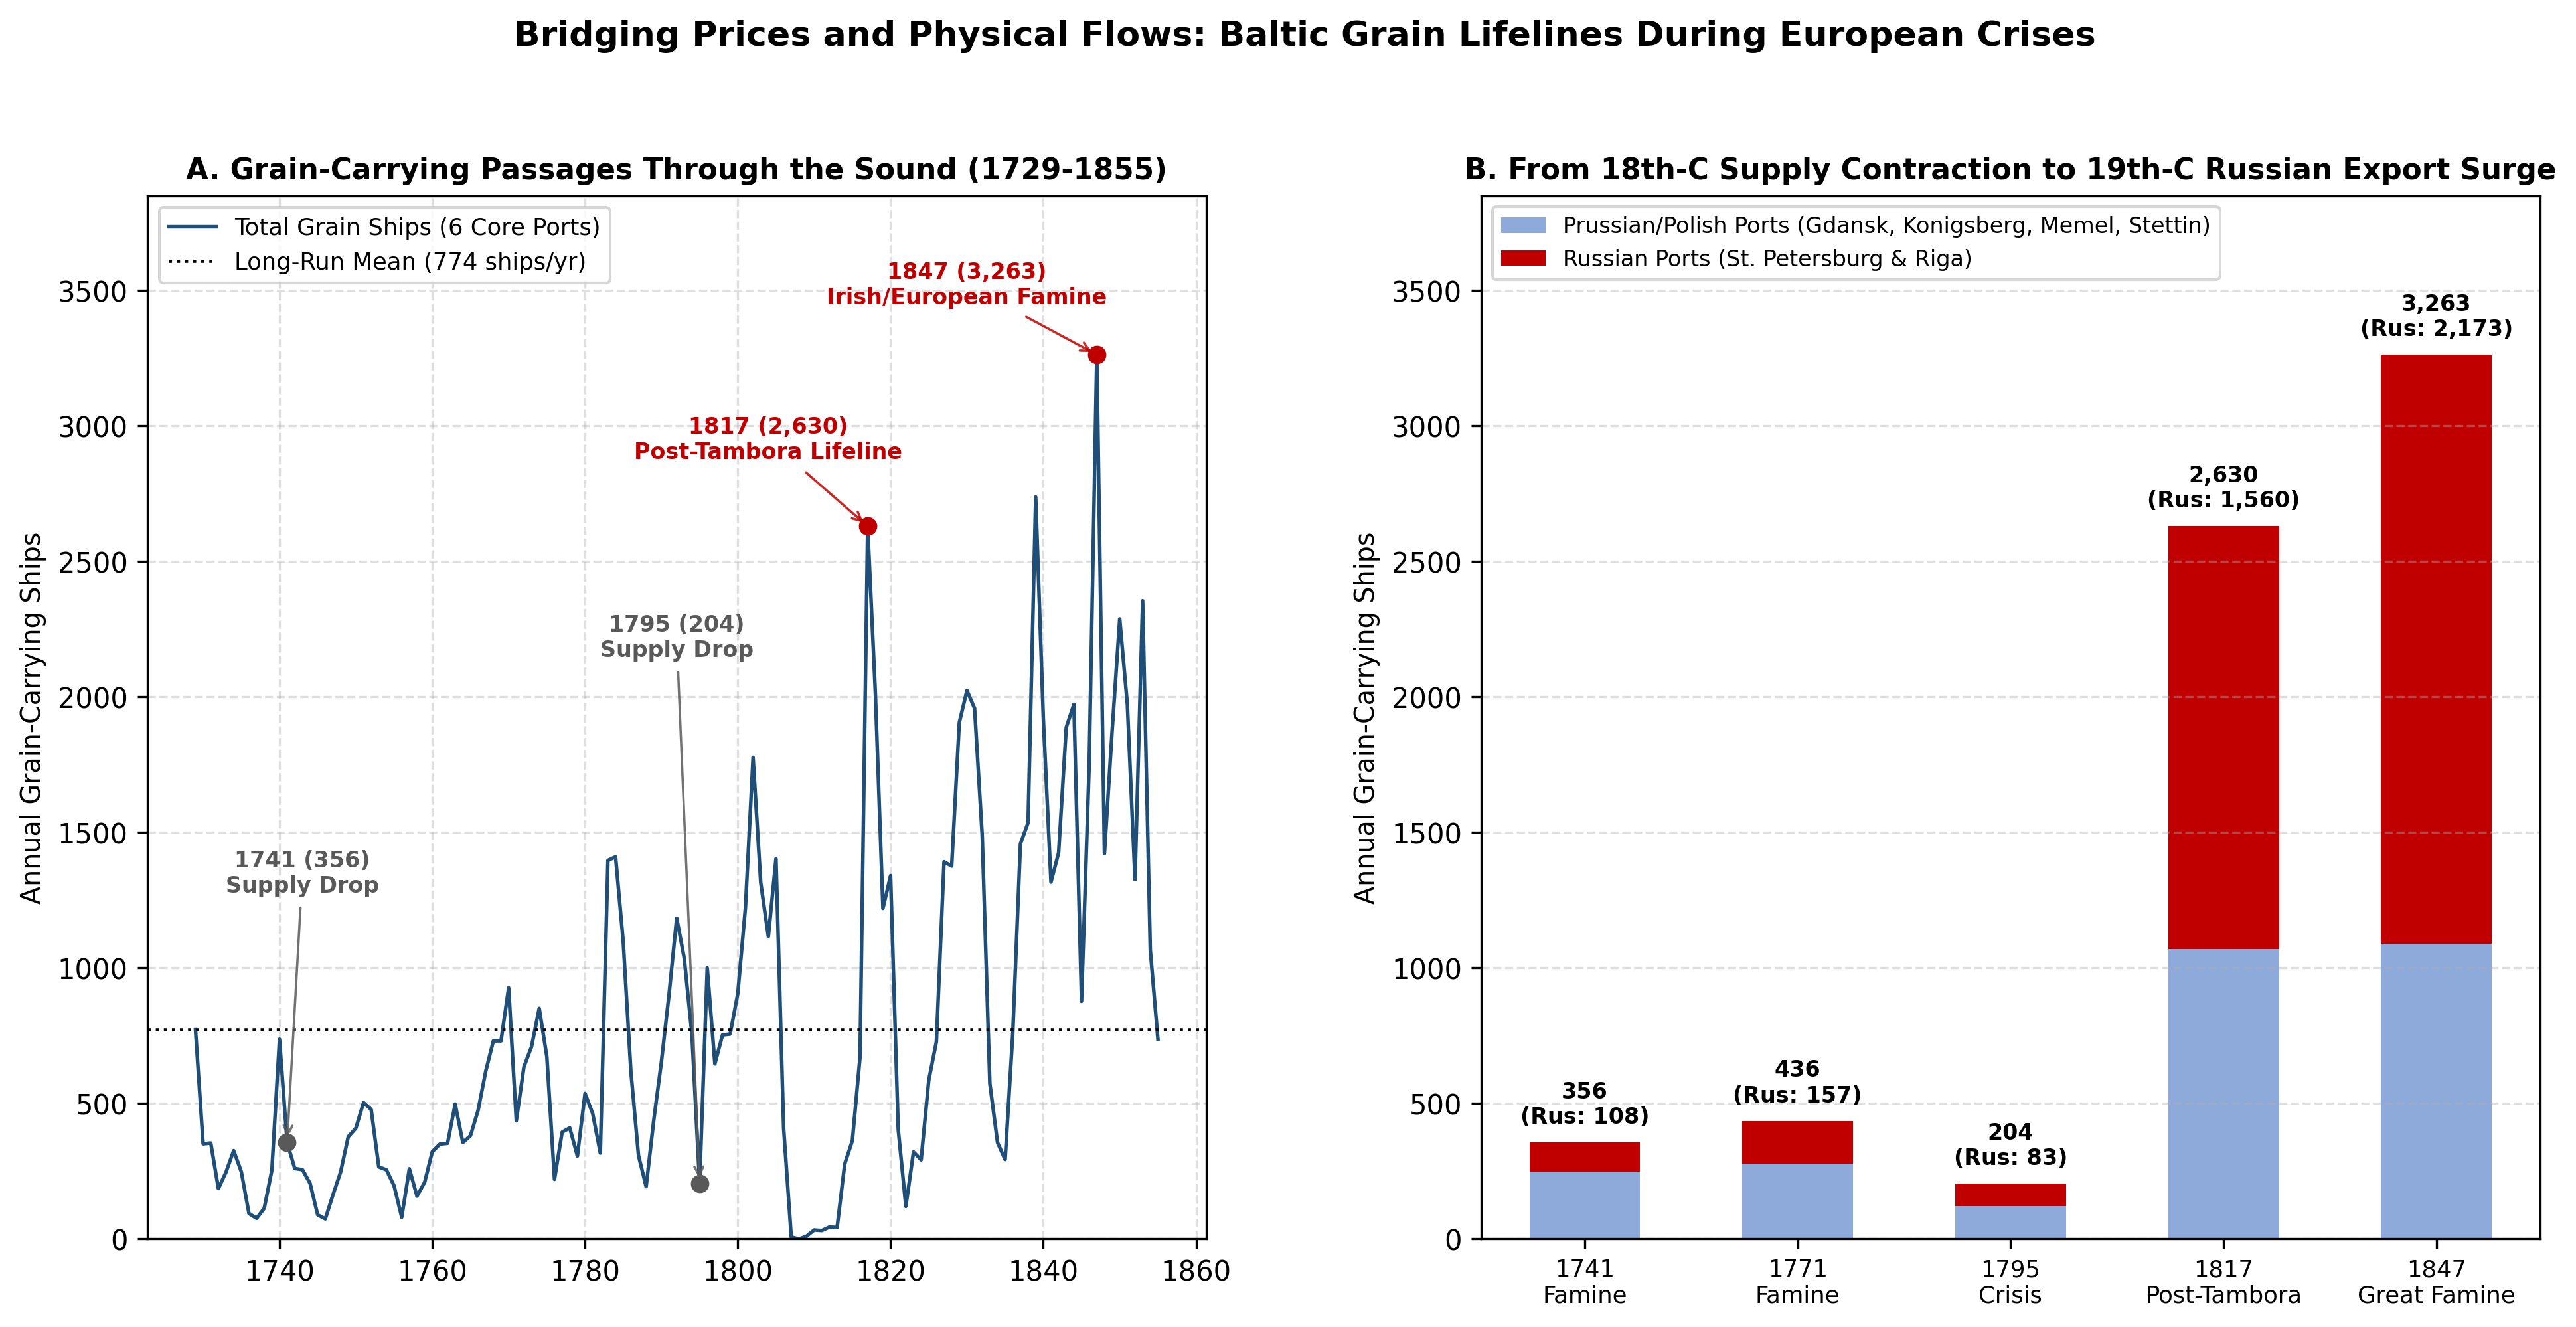
\includegraphics[width=\textwidth]{Figure_3_STRO.png}
\caption{\textbf{Bridging Prices and Physical Flows: Baltic Grain Lifelines During European Crises (1729--1855).} \textbf{A:} Total annual grain-carrying passages across six core ports (Gdansk, Konigsberg, Riga, St.~Petersburg, Memel, Stettin) relative to the long-run mean of 774 ships/year. \textbf{B:} Composition of grain shipments during major European famine crises, contrasting eighteenth-century supply contractions (1741, 1771, 1795) against nineteenth-century Russian export surges (1817, 1847).}
\label{fig:fig3}
\end{figure}
Comparing physical grain shipments across the five acute European subsistence crises identified in our price audit (\href{doi.org}{Avtonomov, 2026}) reveals a fundamental regime shift between the eighteenth and nineteenth centuries:
\begin{itemize}
\item \textbf{Eighteenth-Century Supply Contractions (1741, 1771, 1795):} When European bread prices surged in 1741, 1771, and 1795, physical grain shipments through the Sound \emph{contracted} sharply below the 774-ship mean, falling to 356 ships in 1741 (Gdansk 169, Riga 95, Konigsberg 77), 436 ships in 1771 (Riga 156, Konigsberg 128, Gdansk 124), and just 204 ships in 1795 (Konigsberg 79, Riga 62, Gdansk 42). Eighteenth-century price synchronization was therefore driven by correlated weather shocks and export embargoes that simultaneously reduced exportable surpluses in Eastern Europe.
\item \textbf{Nineteenth-Century Russian Export Lifelines (1817 and 1847):} Following the Napoleonic Wars, the expansion of commercial grain agriculture in the Russian interior and the repeal of the British Corn Laws transformed the eastern Baltic into an elastic supply buffer. During the post-Tambora subsistence crisis of 1817, grain passages surged to 2,630 ships (3.4 times the long-run mean), with Riga (984 ships) and St.~Petersburg (576 ships) surpassing Konigsberg (531) and Gdansk (385). During the European potato and grain famine of 1847, total clearances reached an all-time peak of 3,263 grain ships (4.2 times the mean), led by St.~Petersburg (1,275 grain vessels) and Riga (898).
\end{itemize}
\section{Discussion and Conclusion}
Combining archival pre-auditing with two-tier spectral diagnostics reconciles competing interpretations of early modern Baltic commerce. In peacetime, Baltic maritime integration was neither a homogeneous periphery nor a fully unified market: a North Sea--Southern Baltic commercial arc (Rotterdam, Amsterdam, Konigsberg, Gdansk, Riga, Hull) responded synchronously to annual harvest and mercantile conditions, whereas St.~Petersburg anchored a distinct industrial-naval supply chain linked primarily to Britain. Superimposed on this peacetime structure were powerful geopolitical chokepoint shocks—above all the Continental Blockade of 1808--1812 and the Crimean War of 1854--1855—that temporarily severed direct bilateral flags while triggering rapid neutral-flag substitution.
Most importantly, pairing physical passage counts from \texttt{STRO} with historical price series (\href{doi.org}{Avtonomov, 2026}) clarifies the physical mechanism behind European food crises. Before 1800, sharp price spikes in Western Europe coincided with physical export collapses in the Baltic, confirming that eighteenth-century price co-movement reflected shared supply-side scarcity rather than stabilizing arbitrage. By 1817 and 1847, however, improved interior transport and commercial deepening enabled St.~Petersburg and Riga to dispatch thousands of grain vessels westward at the exact moment of peak Western European scarcity, marking the physical birth of an integrated European grain lifeline.
\section*{Data and Code Availability}
The underlying Sound Toll Registers Online (\texttt{STRO}) dataset is publicly available via the University of Groningen and DANS (\url{soundtoll.nl}). All archival pre-auditing scripts, orthographic normalization dictionaries, reproducible Python/Jupyter code, and LaTeX source files for this study are openly archived on GitHub at \url{github.com/avtonomov-petr/baltic-sound-toll-anatomy}.
\appendix
\section{Mathematical Specification of the Auditing Protocol}
Let $X_{t,j} \ge 0$ denote the deduplicated count of outbound ship passages from port $j \in {1,\dots,N}$ in year $t \in {1722,\dots,1856}$. To accommodate zero-passage blockade years without arbitrary row deletion, we compute annual log-growth rates $y_{t,j} = \ln(1 + X_{t,j}) - \ln(1 + X_{t-1,j})$ over $M = 134$ transitions and standardize each column to zero mean and unit variance, $Z_{t,j} = (y_{t,j} - \bar{y}j)/s_j$. Applying thin singular value decomposition $Z = U \Sigma V^\top$ yields orthonormal temporal scores $u_k \in \mathbb{R}^M$ and port loadings $v_k \in \mathbb{R}^N$. Energy dispersion across time and ports is quantified by normalized participation ratios:
\begin{equation}
\mathrm{PR}(u_1) = \frac{\left(\sum_{t=1}^M u_{t,1}^4\right)^{-1} - 1}{M - 1} , \qquad
\mathrm{PR}(v_1) = \frac{\left(\sum_{j=1}^N v_{j,1}^4\right)^{-1} - 1}{N - 1} .
\end{equation}

To test for structural regime breaks without imposing prior historical dates, we construct a symmetric $k$-nearest-neighbor Gaussian affinity graph ($k=8$, bandwidth $\sigma$ set to the median pairwise Euclidean distance among rows of $Z$) and compute the Fiedler eigenvector $\psi_2$ of the normalized graph Laplacian $L_{\mathrm{sym}} = I - D^{-1/2} A D^{-1/2}$. Candidate split points $\tau \in [15, M-15]$ are evaluated via two-sided Mann--Whitney $U$ tests comparing ${\psi_{2,t}}{t \le \tau}$ against ${\psi{2,t}}_{t > \tau}$.
\begin{thebibliography}{99}
\bibitem{Avtonomov2026}
Avtonomov, P. (2026). Crisis echoes or arbitrage? Selective co-movement and integration of the Atlantic grain market, 1729--1914. \emph{Zenodo Preprint}. \url{https://doi.org/10.5281/zenodo.24436177}


\bibitem{Bang1906}
Bang, N. E., \& Korst, K. (1906--1953). \emph{Tabeller over Skibsfart og Varetransport gennem Øresund, 1497--1783} (Vols.\ 1--7). Gyldendal.

\bibitem{Kotilaine2005}
Kotilaine, J. T. (2005). \emph{Russia's foreign trade and economic expansion in the seventeenth century: Windows on the world}. Brill.

\bibitem{Scheltjens2015}
Scheltjens, W. (2015). \emph{Dutch deltas: Emergence, functions and structure of the Low Countries' maritime transport system, ca.\ 1300--1850}. Brill.

\bibitem{vanTielhof2002}
van Tielhof, M. (2002). \emph{The 'Mother of all Trades': The Baltic grain trade in Amsterdam from the late 16th to the early 19th century}. Brill.

\bibitem{Veluwenkamp2018}
Veluwenkamp, J. W., \& Scheltjens, W. (Eds.). (2018). \emph{Early modern shipping and trade: Novel approaches using Sound Toll Registers Online}. Brill.

\bibitem{Wallerstein1980}
Wallerstein, I. (1980). \emph{The modern world-system II: Mercantilism and the consolidation of the European world-economy, 1600--1750}. Academic Press.

\end{thebibliography}

\section*{Figure Alt Text}
\begin{itemize}
\item \textbf{Figure 1 Alt Text:} Four-panel chart of Baltic port trajectories, blockade shocks, and peacetime decomposition.
\item \textbf{Figure 2 Alt Text:} Stacked bar chart of port commodity specialization and wartime shipmaster flag switching.
\item \textbf{Figure 3 Alt Text:} Time series and stacked bar chart of Baltic grain ships during famines.
\end{itemize}
\end{document}